%% LyX 2.3.0 created this file.  For more info, see http://www.lyx.org/.
%% Do not edit unless you really know what you are doing.
\documentclass[english]{beamer}
\usepackage{lmodern}
\renewcommand{\sfdefault}{lmss}
\renewcommand{\ttdefault}{lmtt}
\usepackage[T1]{fontenc}
\usepackage[latin9]{inputenc}
\usepackage{amsmath}
\usepackage{amssymb}
\usepackage{graphicx}
\usepackage[all]{xy}

\makeatletter
%%%%%%%%%%%%%%%%%%%%%%%%%%%%%% Textclass specific LaTeX commands.
% this default might be overridden by plain title style
\newcommand\makebeamertitle{\frame{\maketitle}}%
% (ERT) argument for the TOC
\AtBeginDocument{%
  \let\origtableofcontents=\tableofcontents
  \def\tableofcontents{\@ifnextchar[{\origtableofcontents}{\gobbletableofcontents}}
  \def\gobbletableofcontents#1{\origtableofcontents}
}

%%%%%%%%%%%%%%%%%%%%%%%%%%%%%% User specified LaTeX commands.
\usetheme{Warsaw}
\usepackage{svg}
% or ...

\setbeamercovered{transparent}
% or whatever (possibly just delete it)
\usepackage{etoolbox}
\setbeamertemplate{headline}{%
\leavevmode%
  \hbox{%
    \begin{beamercolorbox}[wd=\paperwidth,ht=2.5ex,dp=1.125ex]{palette quaternary}%
    \insertsectionnavigationhorizontal{\paperwidth}{}{\hskip0pt plus1filll}
    \end{beamercolorbox}%
  }
}
\addtobeamertemplate{navigation symbols}{}{%
    \usebeamerfont{footline}%
    \usebeamercolor[fg]{footline}%
    \hspace{1em}%
    \insertframenumber/\inserttotalframenumber
}
\usepackage{tikz}
\usetikzlibrary{shapes,arrows}
\tikzstyle{triangle}=[fill=blue!20, regular polygon, regular polygon sides=3, draw=black!40]


\makeatother

\usepackage{babel}
\begin{document}

\title[Signatures and models for syntax and operational semantics]{Signatures and models for syntax and operational semantics in the
presence of variable binding}

\author{Ambroise LAFONT\inst{1}}

\institute[IMT]{\inst{1}DAPI\\
IMT Atlantique}

\date[2019]{PhD, 2019}

\makebeamertitle

%\pgfdeclareimage[height=0.5cm]{institution-logo}{institution-logo-filename}
%\logo{\pgfuseimage{institution-logo}}

\AtBeginSubsection[]{%
  \frame<beamer>{ 
    \frametitle{Outline}   
    \tableofcontents[currentsection,currentsubsection] 
  }
}
\AtBeginSection[]{%
  \frame<beamer>{ 
    \frametitle{Outline}   
    \tableofcontents[currentsection,currentsubsection] 
  }
}

%\beamerdefaultoverlayspecification{<+->}

\global\long\def\redr#1#2#3{#2\xrightarrow{#1}#3}
\global\long\def\monsubst#1{[#1]}

\global\long\def\bind{\mathsf{{bind}}}

\robustify{\redr}\robustify{\monsubst}
\begin{frame}{Outline}

\tableofcontents{}

\end{frame}

\section{Reduction monads}

\begin{frame}{Ingredients}

\begin{itemize}
\item Programming languages (PLs) as graphs
\begin{itemize}
\item (\textbf{Syntax}) vertices = terms 
\item (\textbf{Semantics}) arrows = reductions between terms
\end{itemize}
\item Parallel substitution: variables $\mapsto$ terms
\begin{itemize}
\item monads and modules over them
\end{itemize}
\item (untyped PLs)
\end{itemize}
\begin{example}
$\lambda$-calculus with $\beta$-reduction
\[
S,T\quad::=x|S\,T|\lambda x.S
\]
\[
\redr{\beta}{(\lambda x.t)\,u}{t[x\mapsto u]}\qquad+\quad\text{congruences}
\]
modulo $\alpha$-equivalence, e.g. 
\[
\lambda x.x=\lambda y.y
\]
\end{example}

\end{frame}
%

\subsection{Graphs}
\begin{frame}{PLs as graphs}

\framesubtitle{Example: $\lambda$-calculus with $\beta$-reduction}

\begin{tikzpicture}[->,draw=blue,>=latex,every edge/.append style = { text=blue}]
%\tikzset{>=latex}

\node (v1) at (-6,11) {$(\lambda x.x\ y)\ \mathsf{id}$};
\node (v2) at (-2,10) {$\mathsf{id}\ y$};
\node (Omega) at (-5,7) {$\Omega$};
  
\node (Omega2) at (1,9) {$\Omega\ \Omega$};
\draw  (Omega) edge[loop, looseness=20] node[sloped, above] {$\beta$}(Omega);
\draw  (v1) edge node[sloped, above] {$\beta$}(v2);
\draw  (Omega2) edge[loop, looseness=20] node[sloped, above] {$\beta\ \Omega$}(Omega2);
\draw  (Omega2) edge[loop below, looseness=40] node[sloped, below] {$\Omega\ \beta$}(Omega2);
\node (v3) at (-1,7.5) {$y$};
\draw  (v2) edge node[sloped, above] {$\beta$}(v3);
\end{tikzpicture}


\vspace{-1em}
\begin{columns}
%

\column{\dimexpr\paperwidth-35pt}
\begin{itemize}
\item (\textbf{Syntax}) vertices = terms 
\item (\textbf{Semantics}) arrows = reductions (dedicated syntax: Cf labels)
\end{itemize}
\end{columns}

\end{frame}
%
\begin{frame}{Graphs}

\framesubtitle{Definition}

Graph = a quadruple $(A,V,\sigma,\tau)$ where 
\[
\xymatrix{A\ar@<+.5ex>[r]^{\sigma}\ar@<-0.5ex>[r]_{\tau} & V}
\]

\[
A=\{\text{arrows}\}\qquad\qquad V=\{\text{vertices}\}
\]

\[
\begin{array}{rcl}
\sigma: & {\color{blue}A} & \to V\\
 & {\color{blue}t\xrightarrow{r}u} & \mapsto t
\end{array}\qquad\begin{array}{rcl}
\tau: & {\color{blue}A} & \to V\\
 & {\color{blue}t\xrightarrow{r}u} & \mapsto u
\end{array}
\]

\[
\sigma(r)\xrightarrow{r}\tau(r)
\]

\end{frame}
%
\begin{frame}{PLs as bipartite graphs}

\framesubtitle{Example: $\lambda$-calculus cbv with big-step operational semantics}
\begin{itemize}
\item term $\rightarrow$ value
\item variables = placeholders for values
\end{itemize}

\bigskip

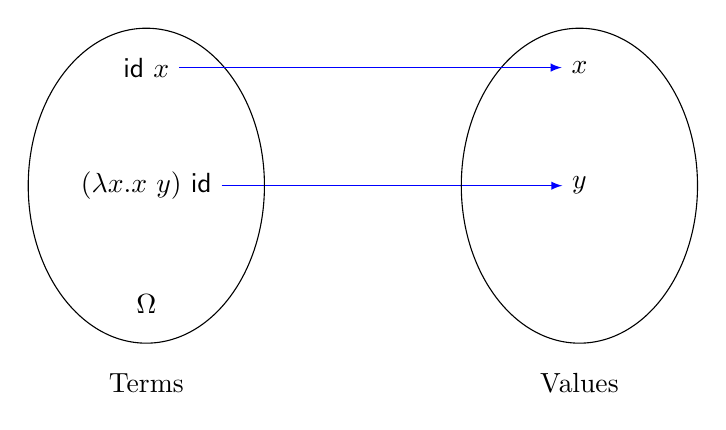
\begin{tikzpicture}[->,draw=blue,>=latex,every edge/.append style = { text=blue}]
%\tikzset{>=latex}

\node (v1) at (-5.5,11) {$(\lambda x.x\ y)\ \mathsf{id}$};
\node (v2) at (0,11) {$y$};
\node (w1) at (-5.5,12.5) {$\mathsf{id}\ x$};
\node (w2) at (0,12.5) {$x$};
\node (Omega) at (-5.5,9.5) {$\Omega$};


\draw  (v1) edge (v2);
\draw[black]  (-5.5,11) ellipse (1.5 and 2);
\draw[black]  (0,11) ellipse (1.5 and 2);
\node at (-5.5,8.5) {Terms};
\node at (0,8.5) {Values};
\draw  (w1) edge (w2); 
\end{tikzpicture}

\end{frame}
%
\begin{frame}{Bipartite graphs}

\framesubtitle{Definition}

Bipartite graph = a quadruple $(A,V_{1},V_{2},\partial)$ where 
\[
V_{1}\xleftarrow{\sigma}A\xrightarrow{\tau}V_{2}
\]

\[
A=\{\text{arrows}\}\qquad\qquad\begin{aligned}V_{1} & =\{\text{vertices in first group}\}\\
V_{2} & =\{\text{vertices in second group}\}
\end{aligned}
\]

\vspace{1em}

For simplicity, we focus on the particular case of \textbf{graphs}:
$V_{1}=V_{2}$.
\end{frame}
%

\subsection{Substitution}

\begin{frame}{Parallel substitution}

\framesubtitle{Syntax comes with substitution}

\framesubtitle{}
\begin{columns}
%

\column{\dimexpr\paperwidth-20pt}

terms (e.g. $\lambda$-terms) = trees with free variables as (distinguished)
leaves.

\end{columns}

\vspace{1em}

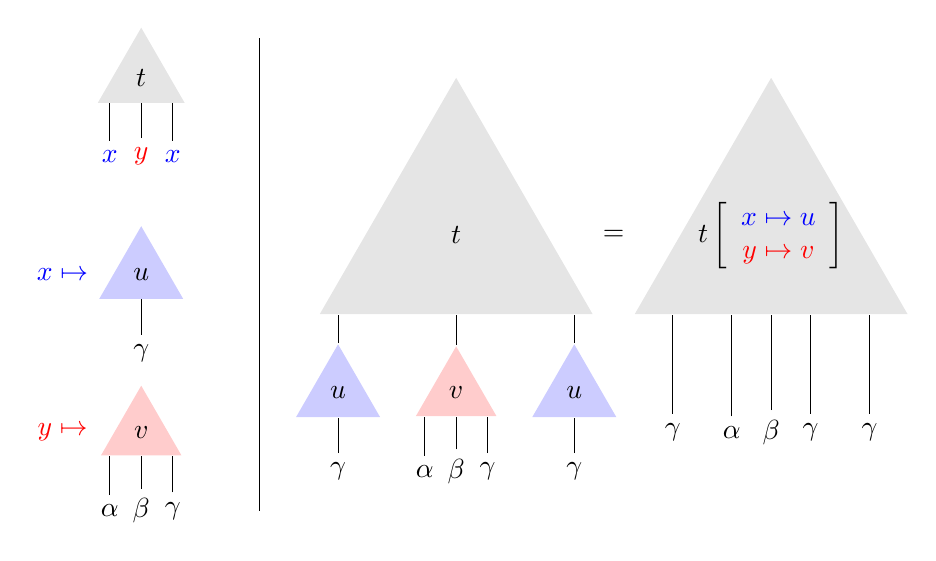
\begin{tikzpicture}[  triangle/.style = 
{fill=blue!20, regular polygon, regular polygon sides=3}]



%
\node[triangle, fill=gray!20] (v1) at (-6.5,5) {$t$};
\node (x1) at (-6.9,4) {$\textcolor{blue}{x}$};
\node (xn) at (-6.1,4) {$\textcolor{blue}{x}$}; 
\node (xi) at (-6.5,4) {$\textcolor{red}{y}$}; 
\draw  (x1.north) edge (x1.north|-v1.south);
\draw  (xn.north) edge (xn.north|-v1.south);
\draw  (xi.north) edge (xi.north|-v1.south);

\node[triangle, fill=blue!20] (u) at (-6.5,2.5) {$u$};
% \node (y1) at (0.1,3.5) {$\alpha$};
% \node (yn) at (0.9,3.5) {$\gamma$}; 
\node (yi) at (-6.5,1.5) {$\gamma$}; 
%\draw  (y1.north) edge (y1.north|-u.south);
%\draw  (yn.north) edge (yn.north|-u.south);
\draw  (yi.north) edge (yi.north|-u.south);

\node[triangle, fill=red!20] (v) at (-6.5,0.5) {$v$};
\node (y11) at (-6.9,-0.5) {$\alpha$};
\node (y1i) at (-6.5,-0.5) {$\beta$}; 
\node (y1n) at (-6.1,-0.5) {$\gamma$}; 
%\node (y1i) at (3.5,0) {$\dots$}; 
\draw  (y11.north) edge (y11.north|-v.south);
\draw  (y1n.north) edge (y1n.north|-v.south);
\draw  (y1i.north) edge (y1i.north|-v.south);

\node[triangle, fill=blue!20] (u2) at (-4,1) {$u$};
%\node (y1) at (2.1,1.5) {$\alpha$};
%\node (yn) at (2.9,1.5) {$\gamma$}; 
\node (yi) at (-4,0) {$\gamma$}; 
%\draw  (y1.north) edge (y1.north|-u2.south);
%\draw  (yn.north) edge (yn.north|-u2.south);
\draw  (yi.north) edge (yi.north|-u2.south);
%

\node[triangle, fill=red!20] (v) at (-2.5,1) {$v$};
\node (y11) at (-2.9,0) {$\alpha$};
\node (y1n) at (-2.1,0) {$\gamma$}; 
\node (y1i) at (-2.5,0) {$\beta$}; 
%\node (y1i) at (3.5,0) {$\dots$}; 
\draw  (y11.north) edge (y11.north|-v.south);
\draw  (y1n.north) edge (y1n.north|-v.south);
\draw  (y1i.north) edge (y1i.north|-v.south);

\node[triangle, fill=blue!20] (u1) at (-1,1) {$u$};
%\node (y1) at (5.1,1.5) {$\alpha$};
%\node (yn) at (5.9,1.5) {$\gamma$}; 
\node (yi) at (-1,0) {$\gamma$}; 
%\draw  (y1.north) edge (y1.north|-u1.south);
%\draw  (yn.north) edge (yn.north|-u1.south);
\draw  (yi.north) edge (yi.north|-u1.south);

\node at (-7.5,2.5) {$\textcolor{blue}{x\mapsto}$};
\node at (-7.5,0.5) {$\textcolor{red}{y\mapsto}$};

%
\node[triangle, fill=gray!20, minimum size=4cm] (v1) at (-2.5,3) {$t$};
%
 
\draw  (u1.north) edge (u1.north|-v1.south);
\draw  (u2.north) edge (u2.north|-v1.south);
\draw  (v.north) edge (v.north|-v1.south);

% \node[triangle, fill=gray!20] (v1) at (0,8) 
% {$t\left[ \begin{array}{c} \textcolor{blue}{x \mapsto u} \\ 
% \textcolor{red}{y \mapsto  v}\end{array}\right]  $};

\node[triangle, fill=gray!20, 
minimum size=4cm,
label=center:{$t\left[ \begin{array}{c} \textcolor{blue}{x \mapsto u} \\ 
\textcolor{red}{y \mapsto  v}\end{array}\right]  $}] (v1) at (1.5,3) {};

\node (v2) at (0.25,0.5) {$\gamma$};
\draw  (v2.north) edge (v2.north|-v1.south);

\node (v2) at (1,0.5) {$\alpha$};
\draw  (v2.north) edge (v2.north|-v1.south);

\node (v2) at (1.5,0.5) {$\beta$};
\draw  (v2.north) edge (v2.north|-v1.south);

\node (v2) at (2,0.5) {$\gamma$};
\draw  (v2.north) edge (v2.north|-v1.south);

\node (v2) at (2.75,0.5) {$\gamma$};
\draw  (v2.north) edge (v2.north|-v1.south);


% \node (v2) at (2,5) {$\gamma$};
% \draw  (v2.north) edge (v2.north|-v1.south);
% \node (v2) at (2.5,5) {$\gamma$};
% \draw  (v2.north) edge (v2.north|-v1.south);

\node at (-0.5,3) {$=$};
\draw (-5,5.5) -- (-5,-0.5);
\end{tikzpicture}

\end{frame}
%
\begin{frame}{Parallel substitution made formal}

\framesubtitle{}
\begin{columns}
%

\column{\dimexpr\paperwidth-20pt}
\begin{block}{Free variables indexing}
\[
X\mapsto\{\text{terms taking free variables in \ensuremath{X}}\}
\]

\vspace{-0.5em}
\begin{exampleblock}{Example: $\lambda$-calculus}

\vspace{-1em}

\[
L(\{x,y\})=\left\{
\begin{aligned}
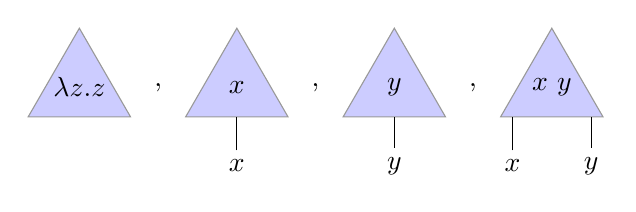
\begin{tikzpicture}
 % \node[triangle, label=center:$\lambda z.z$, minimum size=1.5cm] at (-10.5,4.5) {};
%  \node[anchor=west] at (-9.5,4.5) {$\in L(\emptyset)=\{ \text{closed terms} \}$};
\node[triangle, label=center:$\lambda z.z$, minimum size=1.5cm] at (-16.5,3) {};
%/*
 \node[triangle, label=center:$x$, minimum size=1.5cm] (u) at (-14.5,3) {};
\node (yi) at (-14.5,2) {$x$}; 
\draw  (yi.north) edge (yi.north|-u.south);
\node[triangle, label=center:$y$, minimum size=1.5cm] (u) at (-12.5,3) {};
\node (yi) at (-12.5,2) {$y$}; 
\draw  (yi.north) edge (yi.north|-u.south);
%*/
\node[triangle, label=center:$x\ y$, minimum size=1.5cm] (u) at (-10.5,3) {};
\node (yi) at (-11,2) {$x$}; 
\draw  (yi.north) edge (yi.north|-u.south);
\node (yi) at (-10,2) {$y$}; 
\draw  (yi.north) edge (yi.north|-u.south); 
\node at (-15.5,3) {,};
\node at (-13.5,3) {,};
\node at (-11.5,3) {,};
%\node[anchor=west] at (-9.5,3) {$\in L(\{x,y\})$};
%\node[anchor=east] at (-18.5,3) {$\ L(\{x,y\}) = $};
\end{tikzpicture}
\end{aligned}
,
\dots
\right\}
\]
\end{exampleblock}
\end{block}
%
\begin{block}{Parallel substitution}
For any $f:X\rightarrow L(Y)$,

\vspace{-1em}

\[
\begin{array}{crcl}
\bind_{f}: & L(X) & \rightarrow & L(Y)\\
 & t & \mapsto & t[x\mapsto f(x)]\qquad(\text{or\, }t[f])
\end{array}
\]
\end{block}
\end{columns}

\end{frame}
\global\long\def\fauxtext{of}
%
\begin{frame}{Monads}

\framesubtitle{$\lambda$-calculus as a monad $(L,\bind,\eta)$}

\begin{enumerate}
\item Parallel substitution $(L,\bind)$
\item Variables are terms\vspace{-1em}
\[
\begin{array}{cccc}
\eta_{X}: & X & \rightarrow & L(X)\\
 & x & \mapsto & \begin{aligned}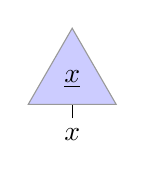
\begin{tikzpicture}\node[triangle](a)at(0,0){\underline{\ensuremath{x}}};\node(b)at(0,-0.7){\ensuremath{x}};\draw(b.north)edge(b.north|-a.south);\end{tikzpicture}\end{aligned}
\end{array}
\]
 
\item Monadics laws:
\[
\underline{x}[f]=f(x)\qquad\qquad t[x\mapsto\underline{x}]=t
\]

+ associativity:
\[
t[f][g]=t\left[x\mapsto f(x)[g]\right]
\]

\end{enumerate}
\end{frame}
%
\begin{frame}{Substitution for semantics}

\framesubtitle{}
\begin{columns}
%

\column{\dimexpr\paperwidth-20pt}

Our notion of PL:
\begin{itemize}
\item \textbf{Syntax}: a monad $(L,\bind,\eta)$
\item \textbf{Semantics}:
\begin{itemize}
\item graphs $\xymatrix{R(X)\ar@<+.5ex>[r]^{\sigma}\ar@<-0.5ex>[r]_{\tau} & L(X)}
$ for each $X$
\[
R(X)=\begin{array}{c}
\text{total set of reductions between}\\
\text{terms taking free variables in \ensuremath{X}}
\end{array}
\]
\item substitution of reduction: variables \textbf{$\mapsto$ $L$-terms}.
\end{itemize}
\[
\dfrac{\redr rtu}{\redr{r\monsubst f}{t\monsubst f}{u\monsubst f}}
\]

\end{itemize}
\end{columns}

\end{frame}
%
\begin{frame}{Substitution for semantics made formal}

\framesubtitle{}

\begin{columns}
%

\column{\dimexpr\paperwidth-50pt}
\begin{block}{$R$ as a \textbf{module} over $L$}

\textrm{For any $f:X\rightarrow\boldsymbol{L}(Y)$,}

\[
\begin{array}{crl}
\bind_{f}: & R(X) & \rightarrow R(Y)\\
 & r & \mapsto r[x\mapsto f(x)]\quad(\text{or }r[f])
\end{array}
\]
s.t.
\[
r[x\mapsto\underline{x}]=r\qquad\qquad r[f][g]=r\left[x\mapsto f(x)[g]\right]
\]

\end{block}
%
\begin{block}{$\sigma$ and $\tau$ as \textbf{$L$-module morphisms}}

\textcolor{blue}{}
\[
\redr{r\monsubst f}{{\color{blue}\sigma(r\monsubst f)}}{{\color{red}\tau(r[f])}}
\]
\[
\text{Then},\quad\dfrac{\redr r{\sigma(r)}{\tau(r)}}{\redr{r\monsubst f}{{\color{blue}\sigma(r)\monsubst f}}{{\color{red}\tau(r)[f]}}}\quad\text{enforces\ensuremath{\quad\begin{aligned}{\color{blue}\sigma(r[f])=\sigma(r)[f]}\\
{\color{red}\tau(r[f])=\sigma(r)[f]}
\end{aligned}
}}
\]
Commutation with substitution $\Leftrightarrow$ Module morphisms
$\sigma,\tau:R\rightarrow L$.
\end{block}
\end{columns}

\end{frame}
%
\begin{frame}{Reduction monads}

\framesubtitle{Definition}

Reduction monad: a quadruple $(L,R,\sigma,\tau)$ s.t.
\begin{itemize}
\item $L$ = monad
\item $R$ = module over $L$
\item $\sigma,\tau:R\rightarrow L$ are $L$-module morphisms.
\end{itemize}
\begin{example}
$\lambda$-calculus with $\beta$-reduction.
\end{example}

\textbf{How can we specify a reduction monad?}
\begin{enumerate}
\item  signature for the (syntactic) operations for the monad;
\item  reduction rules,\textcolor{blue}{{} involving some specified syntactic
operations}.
\end{enumerate}
Use of a general notion of \textbf{signature} managing this \textcolor{blue}{dependency}.

\end{frame}

\section{General signatures}
\begin{frame}{Specify reduction monads}
\end{frame}
%
\begin{frame}{Overview}
\begin{itemize}
\item A signature is a sequence of arities $A_{1},\dots,A_{n}$
\end{itemize}
\end{frame}

\section{Syntax}

\begin{frame}{Overview}
\begin{itemize}
\item Syntax = monad $L$
\item Operations = module morphisms $\Sigma(L)\rightarrow L$
\item 1-signatures specify operations
\item 2-signatures specify operations + equations.
\end{itemize}
\end{frame}
%
\begin{frame}{Operations as module morphisms}

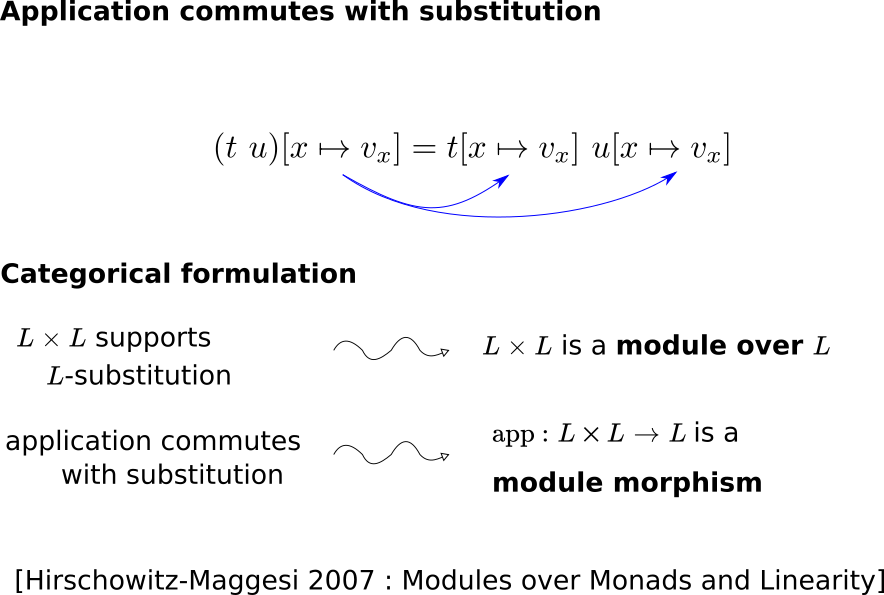
\includegraphics[width=1\textwidth]{images/operations-as-module-morphisms}
\end{frame}
%
\begin{frame}{Examples of modules}

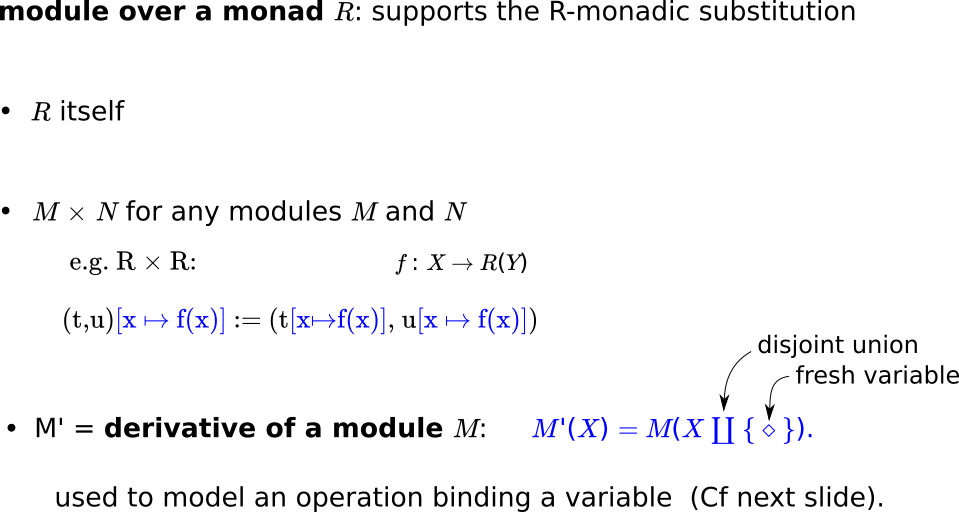
\includegraphics[width=1\textwidth]{images/examples-modules}
\end{frame}
%
\begin{frame}{Operations as module morphisms}

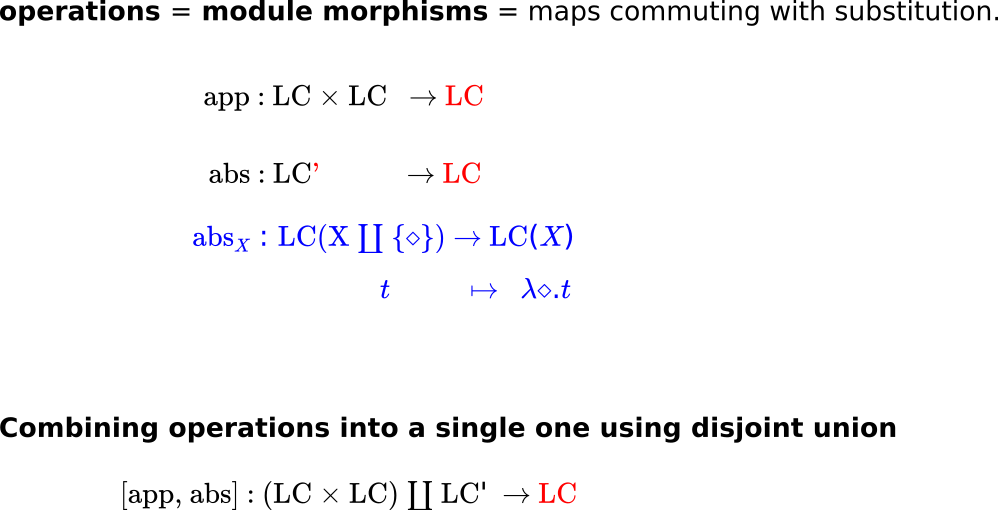
\includegraphics[width=1\textwidth]{images/operations-as-module-morphisms-2}
\end{frame}
%
\begin{frame}{1-signatures and their models}

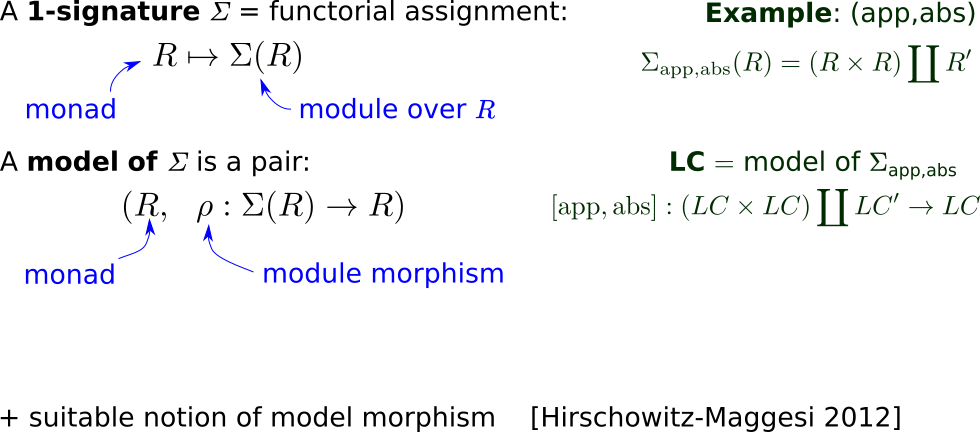
\includegraphics[width=1\textwidth]{images/1-sig_and_their_models}
\end{frame}
%
\begin{frame}{Syntax}

\includegraphics[viewport=0bp 0bp 1024bp 400bp,width=1\textwidth]{slides/syntax}

\end{frame}

\section{Semantics}

\section*{Summary}
\begin{frame}{Summary}
\begin{itemize}
\item The \alert{first main message} of your talk in one or two lines.
\item The \alert{second main message} of your talk in one or two lines.
\item Perhaps a \alert{third message}, but not more than that.
\end{itemize}
\medskip{}

\begin{itemize}
\item Outlook
\begin{itemize}
\item What we have not done yet.
\item Even more stuff.
\end{itemize}
\end{itemize}
\end{frame}

\appendix

\section*{Appendix}

\subsection*{For Further Reading}
\begin{frame}[allowframebreaks]{For Further Reading}

\beamertemplatebookbibitems
\begin{thebibliography}{1}
\bibitem{Author1990}A. Author. \newblock\emph{Handbook of Everything}.\newblock
Some Press, 1990.\beamertemplatearticlebibitems

\bibitem{Someone2002}S. Someone.\newblock On this and that\emph{.}
\newblock\emph{Journal on This and That}. 2(1):50\textendash 100,
2000.
\end{thebibliography}
\end{frame}

\end{document}
